\subsection{Newton’s Fluxions: From Geometry to Motion (1670s)}

  Isaac Newton didn’t just invent calculus: he invented a new way to think about time itself.
  
  In the \textit{Principia}, he draws a sharp distinction between two kinds of time:

  \begin{quote}
  Absolute, true, and mathematical time, of itself, and from its own nature, flows equably without relation to anything external...
  \end{quote}
  
  For Newton, time was like a cosmic river. All motion, all change, all flux happened within this background flow. It didn’t depend on clocks or planets or observers. Time \textit{was} like some divine metronome that ticked in the background.
  
  This view shaped his entire mathematical framework. The derivative—what he called the \textbf{fluxion} was a rate of change \textit{with respect to absolute time}. Every evolving quantity had a speed that happened within the silent rhythm of Newton’s eternal clock.

  Where others saw geometry, Newton saw \textbf{kinematics}. Where others measured lengths, he measured \textbf{change}. And at the center of it all was time—not as an illusion, but as the most real thing in the universe.

  Before Newton, Astronomers charted paths but never asked the deeper question: \textit{how does motion unfold through time?} \textbf{Kinematics} changed that.

  \begin{HistoricalSidebar}{Newton and Augustine --— Time Between Eternity and Motion}

    When Isaac Newton described \textit{absolute time} as flowing “of itself, from its own nature, equably without relation to anything external,” he wasn’t just making a mathematical statement: he was echoing a much older philosophical tradition.

    \medskip
    
    Over a thousand years earlier, \textbf{St. Augustine} grappled with the mystery of time in his \textit{Confessions}. Augustine famously asked:
    
    \begin{quote} \textit{“What then is time? If no one asks me, I know; if I wish to explain it to one that asketh, I know not.”} \end{quote}
    
    For Augustine, time was inseparable from the soul’s perception. He argued that past and future exist only as present memory and anchored in human consciousness. God, by contrast, exists in a timeless eternity where all moments are present at once.

    \medskip
    
    While Augustine located time within the mind’s experience, Newton externalized it. Time, for Newton, was not psychological: it was a universal \textbf{divine framework} set by God Himself. In fact, Newton’s absolute time can be seen as a mathematical counterpart to Augustine’s theological eternity: both are immutable, unaffected by the material world.

    \medskip
    
    But where Augustine saw time as a measure of the soul’s journey through creation, Newton transformed it into a precise, ticking backdrop against which \textit{motion} could be quantified.

    \medskip
    
    \begin{center}
      \begin{tabular}{c c c}
      \textbf{Augustine} &  & \textbf{Newton} \\
      \hline
      Time as inner experience & $\longleftrightarrow$ & Time as cosmic constant \\
      Bound to consciousness   &                      & Independent of observers \\
      Eternity as divine present &                    & Absolute time as divine clockwork \\
      \end{tabular}
      \end{center}
    
    \medskip

    Yet both men agreed on one thing: \textbf{time was real, and it flowed according to divine principles}. For Augustine, those principles were psychological; for Newton, they were mechanical, but still underpinned by creator God.
    
  \end{HistoricalSidebar}
  

    \medskip
    
    Newton stripped away causes and forces and focused only on motion itself. It didn’t ask \textit{why} things moved, only \textit{how fast}, \textit{in what direction}, and \textit{how that changed over time}.

    \textbf{Key Developments:}
    

    \begin{itemize}
      \item \textbf{Galileo Galilei} studied uniformly accelerated motion and laid the groundwork for describing motion using time, distance, and velocity — even before calculus.
      \item \textbf{Isaac Newton} took this further, developing calculus as a tool for describing how quantities change — giving us acceleration, jerk, and higher derivatives as measurable realities.
      \item Kinematics became the scaffolding for Newton’s deeper theory: \textbf{dynamics}, which added force and mass into the mix.
    \end{itemize}
    
    Kinematics was the first major shift in physics to treat time as a variable rather than a stage. It formalized the idea that motion is not just spatial, but \textbf{temporal}. Every modern theory of motion — from relativity to quantum mechanics — builds on this insight.
    
    \begin{quote}
    Kinematics didn’t explain the universe.  It gave us the vocabulary to describe its dance.
    \end{quote}

To Newton, quantities were not static magnitudes, but flowing values—changing continuously with time. Instead of drawing triangles on curves, he imagined how a point moved along a curve, and how its position evolved. This shift—from shape to speed, from geometry to kinematics—transformed the mathematics of the curve into the mathematics of change itself.

He denoted this with a dot over the variable:

\[
\dot{x} = \frac{o}{\bar{o}}
\]

where:

\begin{itemize}
    \item \( o \) is an \textbf{infinitely small increment} of time.  
    \item \( \bar{o} \) is the corresponding change in \( x \).
\end{itemize}


Unlike his predecessors, Newton did not merely approximate motion: he embedded it into the foundations of his system. 
Tangents were consequences of how quantities flowed.

Newton didn’t invent acceleration—that was Galileo, who noticed that falling objects don’t just move; they \textit{accelerate}. 
But Galileo stopped at observation. Newton gave it a cause—and a calculus.
  
\textbf{Step one: Define acceleration in terms of fluxions.}  
Using his own notation, Newton described acceleration as the \textit{fluxion of velocity}, written as:
\[
\dot{v}
\]

\textbf{Step two: Define momentum.}  

He understood that the quantity of motion --— what we now call momentum --- was proportional to mass and velocity:
\[
p = m v
\]

\textbf{Step three: Relate force to the change of momentum.}  

In the \textit{Principia}, Newton writes:

\begin{quote}
\textit{The change of motion is proportional to the motive force impressed.}
\end{quote}

Here, “motion” means momentum. So mathematically:

\[
F = \dot{p}
\]

Now, assuming mass is constant (which Newton generally did), this becomes:

\[
F = \dot{(mv)} = m\dot{v}
\]

\textbf{And there it is.} Not \( F = ma \), but \( F = m\dot{v} \): force as the fluxion of momentum.

\textbf{Galileo saw that velocity changed with time. Newton gave that change a cause—and a law.}

By linking force to motion through fluxions, Newton wasn’t just describing the world. 
He was explaining it—on Earth, in the heavens, and everywhere time flows.


\begin{figure}[H]
\centering
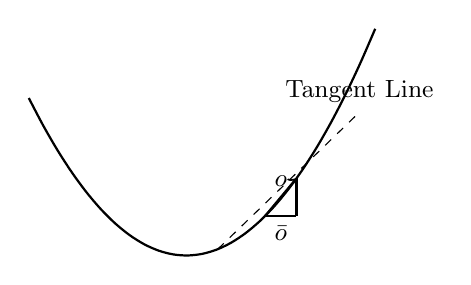
\begin{tikzpicture}[scale=2]
    % Draw the curve
    \draw[thick, domain=-1:1.2, smooth, variable=\x] plot ({\x},{\x*\x});

    % Draw infinitesimal motion
    \draw[->, thick] (0.5, 0.25) -- (0.7, 0.49) node[midway, above] {\small $o$};
    \draw[thick] (0.5, 0.25) -- (0.7, 0.25);
    \draw[thick] (0.7, 0.25) -- (0.7, 0.49);
    \node[below] at (0.6,0.25) {\small $\bar{o}$};
    
    % Draw tangent line
    \draw[dashed] (0.2, 0.04) -- (1.1, 0.91) node[above] {\small Tangent Line};

\end{tikzpicture}

\vspace{0.5em}
\caption{\small Newton's conception of calculus was rooted in geometry and motion. He imagined a point moving along a curve, where the instantaneous rate of change — the fluxion — could be represented as the ratio between an infinitesimal vertical change ($o$) and an infinitesimal horizontal change ($\bar{o}$). The resulting quantity corresponds to the slope of the tangent line at that point. This approach reflects Newton’s view of change as inherently tied to physical movement through time.}
\end{figure}



\begin{figure}[H]
  \centering
  \begin{tikzpicture}[scale=2]
      % Draw the unit circle
      \draw[thick] (0,0) circle (1);
  
      % Pick a point on the circle (45°) and mark it
      \coordinate (P) at ({cos(45)},{sin(45)});
      \fill (P) circle (0.5pt) node[above right] {\small $P$};
  
      % Draw an infinitesimal horizontal increment 'o'
      \coordinate (Hx) at ($(P)-(0.2,0)$);
      \draw[->, thick] (P) -- (Hx) node[midway, above] {\small $o$};
  
      % Draw an infinitesimal vertical increment 'ō' from P
      \coordinate (Vy) at ($(P)-(0,0.2)$);
      \draw[thick] (P) -- (Vy) node[left] {\small $\bar{o}$};
  
      % Draw the tangent line at P (slope = –cos/sin = –1 here)
      \draw[dashed] ($(P)+(-0.5,0.5)$) -- ($(P)+(0.5,-0.5)$)
          node[above right] {\small Tangent Line};
  \end{tikzpicture}
  
  \vspace{0.5em}
  \caption{\small Newton’s infinitesimal “fluxion” on a circle: at point $P$ (here at 45°), the horizontal increment $o$ and vertical increment $\bar{o}$ determine the slope of the tangent (dashed line).}
\end{figure}

